\chapter{El interferómetro de Michelson}\label{ch:b2:michelson}

En 1887 Michelson y Morley desdoblaron en dos un haz de luz, enviaron las
mitades por brazos perpendiculares, las recombinaron y vigilaron las
franjas en busca del desplazamiento que debía producir el movimiento de la
Tierra por el éter: nada se movió, y la física cambió. En 2015 el mismo
instrumento --- dos brazos, ahora de cuatro kilómetros y plegados hasta
mil --- registró una onda gravitacional que cambió sus longitudes en una
milésima del diámetro de un protón. Entre esas dos fechas, el
\omterm{def:b2:michelson:instrument}{interferómetro de Michelson} midió el metro en longitudes de onda, resolvió
rayas espectrales y se convirtió en la herramienta habitual de la óptica
de precisión. Este capítulo lo describe en sus dos configuraciones --- la
cuña de aire y la lámina de caras paralelas --- y muestra cómo sus franjas
miden longitudes, índices y espectros.

\section{El instrumento}

\begin{definition}[El interferómetro de Michelson]\label{def:b2:michelson:instrument}
\index{interferómetro de Michelson}\index{lámina separadora}\index{lámina compensadora}
Una \emph{lámina separadora} $Sp$ --- una placa de vidrio con una cara semirreflectante
--- a \qty{45}{\degree} divide en dos un haz incidente: uno va al
espejo $M_1$ y el otro a $M_2$, ambos perpendiculares a sus haces; tras
la reflexión, cada uno vuelve a $Sp$, donde la mitad se envía hacia el
observador, y allí interfieren las dos mitades. Una \emph{lámina compensadora}
$C$, idéntica a la separadora y paralela a ella, se pone en el brazo
que si no cruzaría el vidrio de la separadora una sola vez, de modo que ambos
haces crucen el mismo espesor de vidrio: la \omterm{thm:b2:two-wave-interference:formula}{diferencia de camino} es entonces una
diferencia pura de caminos en el aire, la misma para toda longitud de onda --- que es
lo que exigen las franjas de luz blanca. Las distancias de los espejos a $Sp$ son $d_1$
y $d_2$; uno de los espejos va montado sobre un tornillo micrométrico y sobre tornillos
de inclinación.
\end{definition}

\begin{proposition}[Montaje equivalente]\label{prop:b2:michelson:equivalent}
\index{cuña de aire (Michelson)}\index{lámina de aire (Michelson)}
Visto desde el observador, el interferómetro equivale al espejo
$M_2$ y a la imagen $M_1'$ de $M_1$ en la separadora: una lámina delgada de aire
entre dos superficies reflectantes, de espesor $e = |d_1 - d_2|$, cuyas
dos reflexiones interfieren (\omterm{prop:b2:two-wave-interference:film}{división de amplitud}):
\begin{itemize}
  \item $M_1' \parallel M_2$: una \emph{lámina de aire} de espesor $e$ --- \omterm{prop:b2:michelson:rings}{anillos de
        igual inclinación}, localizados en el infinito, $\delta = 2e\cos i$;
  \item $M_1'$ ligeramente inclinado un ángulo $\alpha$ respecto de $M_2$: una \emph{cuña de aire}
        --- franjas rectas de igual espesor, localizadas en los
        espejos (cerca de la cuña), $\delta = 2\alpha x$ con incidencia normal,
        separadas $\lambda/2\alpha$.
\end{itemize}
En el \emph{contacto} ($e = 0$, $\alpha = 0$) el campo es uniforme y, para la luz
blanca, es el único lugar donde los colores concuerdan: la ``franja blanca''.
\end{proposition}

\begin{proof}
Plegar el brazo de $M_1$ sobre el de $M_2$ por reflexión en $Sp$ lleva los
dos haces a una misma línea con dos espejos separados $e$; las dos ondas que
vuelven son las reflejadas por las dos caras de la lámina de aire (sin
$\lambda/2$ suplementaria: ambas se reflejan en metal y la separadora las trata
simétricamente, salvo una fase constante que desplaza todo el patrón).
Los resultados de las láminas delgadas de \cref{ch:b2:two-wave-interference} se aplican entonces
con $n = 1$.
\end{proof}

\begin{omfigure}
\begin{tikzpicture}[font=\small, x=1cm, y=1cm, >=Stealth]
  \begin{scope}
    % source and beams
    \fill (-3.6,0) circle (1.5pt); \node[font=\footnotesize] at (-3.6,0.35) {$S$};
    \draw[omDef, thick, ->] (-3.4,0) -- (-0.15,0);
    % splitter at 45 deg
    \draw[thick, fill=omExo!30, rotate around={45:(0,0)}] (-0.08,-1.3) rectangle (0.08,1.3);
    \node[font=\footnotesize] at (0.55,-1.0) {$Sp$};
    % compensadora (paralela, en el brazo hacia M1, junto al brazo vertical)
    \draw[thick, fill=omExo!15, rotate around={45:(0,0.9)}] (-0.06,-0.6) rectangle (0.06,0.6);
    \node[font=\footnotesize] at (0.55,1.3) {$C$};
    % mirrors
    \draw[thick] (-0.9,2.6) -- (0.9,2.6); \fill[pattern=north east lines] (-0.9,2.6) rectangle (0.9,2.75); \node[font=\footnotesize] at (1.3,2.6) {$M_1$};
    \draw[thick] (2.8,-0.9) -- (2.8,0.9); \fill[pattern=north east lines] (2.8,-0.9) rectangle (2.95,0.9); \node[font=\footnotesize] at (2.85,1.25) {$M_2$};
    % beams
    \draw[omDef, thick, ->] (0,0.15) -- (0,2.55); \draw[omDef, thick, ->] (0.15,0) -- (2.75,0);
    \draw[omThm, thick, ->] (-0.2,2.45) -- (-0.2,0.2); \draw[omThm, thick, ->] (2.65,-0.2) -- (0.2,-0.2);
    \draw[omProp, thick, ->] (0,-0.2) -- (0,-2.5);
    \node[omProp, font=\footnotesize] at (0,-2.8) {observador};
    \draw[<->] (0.4,0.4) -- (0.4,2.5) node[midway, right, font=\footnotesize] {$d_1$};
    \draw[<->] (0.4,-0.45) -- (2.7,-0.45) node[midway, below, font=\footnotesize] {$d_2$};
  \end{scope}
  \begin{scope}[xshift=8.4cm]
    \draw[thick] (-1.6,0) -- (1.6,0); \fill[pattern=north east lines] (-1.6,-0.15) rectangle (1.6,0); \node[font=\footnotesize] at (2.0,0) {$M_2$};
    \draw[thick, omDef] (-1.6,0.8) -- (1.6,0.8); \node[omDef, font=\footnotesize] at (2.0,0.8) {$M_1'$};
    \draw[<->] (-1.9,0) -- (-1.9,0.8) node[midway, left, font=\footnotesize] {$e$};
    \node[font=\footnotesize] at (0,-0.6) {lámina de aire: anillos en el infinito};
    \draw[thick] (-1.6,-2.4) -- (1.6,-2.4); \fill[pattern=north east lines] (-1.6,-2.55) rectangle (1.6,-2.4);
    \draw[thick, omDef] (-1.6,-2.35) -- (1.6,-1.75); \node[omDef, font=\footnotesize] at (2.0,-1.8) {$M_1'$};
    \node[font=\footnotesize] at (0,-3.0) {cuña de aire: franjas en los espejos};
  \end{scope}
\end{tikzpicture}

{\small A la izquierda, el \omterm{def:b2:michelson:instrument}{interferómetro de Michelson} --- separadora, \omterm{def:b2:michelson:instrument}{lámina
compensadora}, dos espejos y un haz recombinado hacia el observador. A la derecha, la
lámina de aire equivalente entre $M_2$ y la imagen $M_1'$ de $M_1$, paralela
(anillos) o inclinada (franjas rectas).}
\end{omfigure}

\section{Los dos sistemas de franjas}

\begin{proposition}[Anillos de la lámina de aire]\label{prop:b2:michelson:rings}
\index{anillos de igual inclinación}\index{franjas de Haidinger}
Con $M_1' \parallel M_2$ y una \omterm{prop:b2:two-wave-interference:spatial}{fuente extensa}, el observador (o una lente
de distancia focal $f$ y una pantalla en su plano focal) ve anillos
concéntricos; el anillo del ángulo $i$ tiene el orden $p = 2e\cos i/\lambda$, y son
brillantes los anillos de $p$ entero. El centro tiene el orden más alto, $p_0 =
2e/\lambda$; cerca de él, $\cos i \approx 1 - i^2/2$, así que el $k$-ésimo anillo brillante desde el
centro (contado desde el primero, a $\varepsilon = p_0 - \lfloor p_0\rfloor$
por debajo del orden del centro) tiene el radio
\[
r_k = f\,i_k = f\sqrt{\frac{(k - 1 + \varepsilon)\lambda}e} :
\]
anillos más apretados cuanto mayor es $e$ (más anillos y más finos), que se separan cuando $e \to 0$
hasta que, en el contacto, queda un campo uniforme. Mover un espejo $\lambda/2$ cambia
$p_0$ en una unidad: nace un anillo en el centro (o lo traga) por cada
media longitud de onda de desplazamiento.
\end{proposition}

\begin{proof}
$\delta = 2e\cos i$ para la lámina de caras paralelas (\cref{ch:b2:two-wave-interference},
$n = 1$, sin $\lambda/2$ suplementaria por las dos reflexiones metálicas); $2e(1 - i^2/2) =
(p_0 - k + 1 - \varepsilon)\lambda$ con $2e = p_0\lambda$ da $ei^2 = (k - 1 + \varepsilon)\lambda$.
\end{proof}

\begin{proposition}[Franjas de la cuña de aire]\label{prop:b2:michelson:wedge}
\index{franjas de igual espesor (Michelson)}\index{franjas de Fizeau}
Con $M_1'$ inclinado un ángulo pequeño $\alpha$ y con incidencia casi normal, la
\omterm{thm:b2:two-wave-interference:formula}{diferencia de camino} en el punto de los espejos situado a la distancia $x$ de la
línea de contacto vale $\delta = 2\alpha x$: franjas rectas paralelas a esa línea,
separadas $\lambda/2\alpha$, localizadas en los espejos (se observan enfocando
sobre $M_2$, o se proyectan en una pantalla con una lente que conjugue $M_2$ y la
pantalla). La franja de orden cero está sobre la línea de contacto, la misma para
toda longitud de onda: con luz blanca es blanca (o negra, según
las fases de la separadora), flanqueada por unas pocas franjas coloreadas --- la
firma con la que se encuentra el contacto.
\end{proposition}

\begin{proof}
\omterm{prop:b2:two-wave-interference:film}{Franjas de igual espesor} de una cuña de aire, $e(x) = \alpha x$. Localización:
para una \omterm{prop:b2:two-wave-interference:spatial}{fuente extensa}, los rayos que pasan por un punto dado de la cuña
se recombinan allí, con la misma $\delta$ con incidencia casi normal.
\end{proof}

\begin{omfigure}
\begin{tikzpicture}[font=\small, x=1cm, y=1cm, >=Stealth]
  \begin{scope}
    \foreach \r in {0.35,0.62,0.82,0.98,1.12,1.25,1.37,1.48} \draw[omDef, thick] (0,0) circle (\r);
    \node[font=\footnotesize] at (0,-1.9) {anillos: $r_k \propto \sqrt{k}$};
  \end{scope}
  \begin{scope}[xshift=4.8cm]
    \foreach \x in {-1.4,-1.0,...,1.4} \draw[omDef, thick] (\x,-1.5) -- (\x,1.5);
    \node[font=\footnotesize] at (0,-1.9) {cuña: separación $\lambda/2\alpha$};
  \end{scope}
  \begin{scope}[xshift=10.0cm]
    \begin{axis}[omaxis, axis x line=bottom, axis y line=left, width=5.0cm, height=4.2cm, at={(0,-1.9cm)},
        xlabel={$e$ (mm)}, ylabel={contraste}, xmin=0, xmax=1.2, ymin=0, ymax=1.1, xtick={0,0.29,0.58,0.87}, xticklabels={0,0.29,0.58,0.87}, ytick={0,1}, samples=200,
        xlabel style={at={(axis description cs:0.5,-0.14)}, anchor=north},
        ylabel style={at={(axis description cs:-0.12,0.5)}, rotate=90, anchor=south}]
      \addplot[omThm, thick, domain=0:1.2] {abs(cos(deg(pi*x/0.29)))};
    \end{axis}
  \end{scope}
\end{tikzpicture}

{\small Los dos sistemas de franjas del Michelson y el contraste de
las franjas del doblete del sodio frente al espesor de la lámina: se anula
cada \qty{0.29}{mm} (la primera vez en \qty{0.145}{mm}), cuando las franjas de las dos rayas
están en oposición.}
\end{omfigure}

\section{Medir con el Michelson}

\begin{proposition}[Longitudes, índices, espectros]\label{prop:b2:michelson:measure}
\index{espectroscopia por transformada de Fourier}\index{espectro acanalado}
Contar $N$ franjas que pasan por el centro mientras un espejo se desplaza $\Delta e$
da $\Delta e = N\lambda/2$: longitudes en longitudes de onda (un tornillo micrométrico
calibrado a \qty{0.1}{\micro m}; así se midió el propio metro). Una
lámina transparente de espesor $\ell$ e índice $n$ colocada en un brazo
añade $2(n - 1)\ell$ a $\delta$ y desplaza el patrón $2(n - 1)\ell/\lambda$
franjas: índices (y sus variaciones con la presión o la temperatura,
en una cubeta de gas). Con un doblete de longitudes de onda $\lambda$ y $\lambda + \Delta\lambda$, los
dos sistemas de franjas se desacompasan y se vuelven a acompasar al crecer $e$, y el
contraste se anula cada
\[
\Delta e = \frac{\lambda^2}{2\Delta\lambda} :
\]
el desdoblamiento de rayas próximas. De forma más general, el contraste en
función de $e$ dibuja el espectro de la fuente (el contraste
decae en $e \sim \ell_c/2$): registrar la intensidad en el centro mientras
$e$ barre es la \emph{\omterm{prop:b2:michelson:measure}{espectroscopia por transformada de Fourier}}, el método de
los espectrómetros de infrarrojo.
\end{proposition}

\begin{proof}
El orden en el centro vale $2e/\lambda$; cada raya tiene el suyo. Los dos
sistemas vuelven a coincidir cuando $2e/\lambda - 2e/(\lambda + \Delta\lambda) = 1$, es decir, $2e\Delta\lambda
/\lambda^2 = 1$; están en oposición a mitad de camino. El enunciado general es
la fórmula del contraste de \cref{exo:b2:scalar-light-model:10}.
\end{proof}

\begin{example}[El sodio y el metro]\label{ex:b2:michelson:sodium}
El doblete del sodio ($\Delta\lambda = \qty{0.6}{nm}$ a \qty{589}{nm}): los anillos se borran y
se afilan cada $\Delta e = 589^2/(2 \times 0.6)$ nm $= \qty{0.29}{mm}$ --- una medida clásica
de $\Delta\lambda$ con un pequeño porcentaje de error usando un tornillo. Michelson (1892)
contó las franjas de la raya roja del cadmio a lo largo del metro
patrón: $1\,553\,163.5$ longitudes de onda, la primera atadura entre el
metro y un átomo; hoy el metro se define mediante $c$ y el
segundo, y los interferómetros verifican bloques patrón en producción con precisión de
nanómetros.
\end{example}

\begin{omfigure}
\begin{tikzpicture}
\begin{axis}[omaxis, axis x line=bottom, axis y line=left, width=13.6cm, height=4.4cm,
    xlabel={$e$ (\unit{\micro m})}, ylabel={$I$ en el centro}, xmin=0, xmax=6, ymin=0, ymax=2.3, xtick={0,1,2,3,4,5,6}, ytick=\empty, samples=600,
    xlabel style={at={(axis description cs:0.5,-0.14)}, anchor=north},
    ylabel style={at={(axis description cs:-0.04,0.5)}, rotate=90, anchor=south}]
  \addplot[omDef, thick, domain=0:6] {1+exp(-(x/2.2)^2)*cos(deg(2*pi*x/0.55))};
  \addplot[omThm, thick, dashed, domain=0:6] {1+exp(-(x/2.2)^2)};
  \addplot[omThm, thick, dashed, domain=0:6] {1-exp(-(x/2.2)^2)};
\end{axis}
\end{tikzpicture}

{\small La intensidad en el centro de los anillos a medida que crece el espesor de la
lámina, para una fuente de \omterm{prop:b2:scalar-light-model:coherence}{longitud de coherencia} finita: las franjas se apagan en
$e \sim \ell_c/2$; la envolvente es la transformada de Fourier del espectro.}
\end{omfigure}

\begin{remark}[Los brazos que no midieron nada y los que midieron una onda]\label{rem:b2:michelson:history}
\index{experimento de Michelson--Morley}\index{detector de ondas gravitacionales}
Michelson y Morley esperaban que la velocidad $v$ de la Tierra por el
éter cambiara el tiempo de ida y vuelta por el brazo paralelo a ella en
$(L/c)(v/c)^2$ respecto del brazo perpendicular, un desplazamiento de franjas de
$2L(v/c)^2/\lambda \approx 0.4$ franjas para $L = \qty{11}{m}$ y $v = \qty{30}{km/s}$;
girar el aparato debería haber movido el patrón en esa cantidad.
Podían ver $0.01$ franjas; no vieron nada. Los \omterm{rem:b2:michelson:history}{detectores de ondas
gravitacionales} de hoy son Michelson con brazos de \qty{4}{km}, con la luz rebotando
unas trescientas veces en cada uno y un láser lo bastante estable como para leer un
cambio de longitud de brazo $\Delta L/L \sim 10^{-21}$ --- $10^{-18}$ m, una milésima
de protón --- frente al ruido del movimiento sísmico y de los propios
fotones.
\end{remark}

\begin{method}[Cómo usar un Michelson]\label{met:b2:michelson:method}
(1) Identifíquese la configuración: lámina de caras paralelas (anillos en el infinito;
obsérvese con una lente o con el ojo al infinito) o cuña (franjas en los
espejos; enfóquese sobre $M_2$). (2) Escríbase $\delta = 2e\cos i$ o $2\alpha x$ y el
orden. (3) Tradúzcase cada medida a franjas: $\Delta e = N\lambda/2$,
$2(n - 1)\ell$ para una lámina, $\lambda^2/2\Delta\lambda$ para un doblete. (4) Úsese la
posición de contacto ($e = 0$, franja blanca) como referencia absoluta;
téngase en cuenta que los radios de los anillos \emph{disminuyen} al crecer $e$. (5) Límites
de coherencia: los anillos se ven mientras $2e < \ell_c$; la cuña exige
incidencia casi normal.
\end{method}

\section{Ejercicios}

\begin{exercise}[$\star$]\label{exo:b2:michelson:1}
Un Michelson con luz de sodio ($\lambda = \qty{589}{nm}$): se desplaza el espejo
\qty{0.10}{mm}: número de anillos que pasan por el centro; desplazamiento
correspondiente a $250$ franjas; precisión sobre $e$ si puede leerse una décima
de franja.
\end{exercise}

\begin{exercise}[$\star$]\label{exo:b2:michelson:2}
Lámina de caras paralelas de espesor $e = \qty{0.50}{mm}$, lente $f = \qty{1.0}{m}$, $\lambda =
\qty{589}{nm}$: orden en el centro; ¿es brillante el centro? Radios de los
tres primeros anillos brillantes; ¿qué les ocurre a los anillos si $e$ se reduce
a \qty{0.05}{mm}?
\end{exercise}

\begin{exercise}[$\star$]\label{exo:b2:michelson:3}
Cuña de aire con $\alpha = \qty{1.0e-4}{rad}$, $\lambda = \qty{633}{nm}$: separación de las franjas;
número de franjas en \qty{2}{cm} de espejo; se dobla el ángulo de la cuña:
¿qué ocurre? ¿Cómo se encuentra el contacto con luz blanca?
\end{exercise}

\begin{exercise}[$\star$]\label{exo:b2:michelson:4}
Se inserta una placa de vidrio de \qty{0.10}{mm} de espesor en un brazo: desplazamiento de franjas para
$n = 1.52$ a \qty{589}{nm}; el desplazamiento se mide con $0.2$ franjas de precisión: precisión
sobre $n$. ¿Por qué no podría hacerse la misma medida con luz blanca
si la placa midiera \qty{1}{cm}?
\end{exercise}

\begin{exercise}[$\star\star$]\label{exo:b2:michelson:5}
\emph{Doblete del sodio.} (a) Espesor $e$ entre dos desapariciones
sucesivas de los anillos, para $\Delta\lambda = \qty{0.597}{nm}$. (b) Un estudiante
mide $17$ desapariciones en \qty{5.00}{mm}: $\Delta\lambda$ y su precisión.
(c) Órdenes de las dos rayas en $e = \qty{0.29}{mm}$: compruébese que difieren en
$\tfrac12$. (d) ¿Por qué no es nunca exactamente nulo el contraste (las dos rayas tienen
intensidades en la razón $2 : 1$)? Contraste mínimo.
\end{exercise}

\begin{exercise}[$\star\star$]\label{exo:b2:michelson:6}
\emph{Índice del aire.} Se hace el vacío en una cubeta de \qty{10.0}{cm} de un brazo y luego
se llena despacio de aire a \qty{1}{bar}; pasan $94$ franjas ($\lambda = \qty{589}{nm}$).
(a) $n - 1$ del aire. (b) Franjas que pasan por un cambio del \qty{1}{\%} de
presión; coeficiente de temperatura si $n - 1 \propto \rho$. (c) ¿Por qué importa esto
para la estabilidad de cualquier interferómetro en el aire? (d) Precisión sobre
$n - 1$ a partir de una décima de franja.
\end{exercise}

\begin{exercise}[$\star\star$]\label{exo:b2:michelson:7}
\emph{\omterm{prop:b2:scalar-light-model:coherence}{Longitud de coherencia}.} Con una lámpara de mercurio de baja presión (raya verde,
\qty{546}{nm}, de \qty{0.01}{nm} de anchura) los anillos se apagan al crecer $e$. (a) \omterm{prop:b2:scalar-light-model:coherence}{Longitud
de coherencia}; espesor $e$ para el que el contraste se vuelve despreciable. (b) Lo mismo
con una lámpara de alta presión ($\Delta\lambda = \qty{1}{nm}$). (c) Con un láser de He--Ne
($\Delta\nu = \qty{1}{MHz}$): ¿pueden verse todavía anillos con $e = \qty{10}{m}$? (d) ¿Qué
limita las franjas de luz blanca a $\pm2$ órdenes en torno al contacto?
\end{exercise}

\begin{exercise}[$\star\star$]\label{exo:b2:michelson:8}
\emph{\omterm{def:b2:michelson:instrument}{Lámina compensadora}.} Sin $C$, un haz cruza el vidrio de la
separadora ($e_g = \qty{5}{mm}$, $n = 1.52$) tres veces y el otro una sola. (a)
\omterm{def:b2:scalar-light-model:path}{Camino óptico} suplementario; ¿puede compensarse moviendo un espejo para
luz monocromática? (b) ¿Por qué no para luz blanca (dispersión: $n$
varía $0.01$ en el visible)? (c) ¿Qué tolerancia en el
paralelismo de $C$ y $Sp$ conserva la franja blanca (tómese una diferencia
residual de espesor $< \qty{0.3}{\micro m}$)? (d) Las separadoras modernas son
películas finas o cubos: ¿por qué es entonces innecesaria $C$?
\end{exercise}

\begin{exercise}[$\star\star$]\label{exo:b2:michelson:9}
\emph{Michelson--Morley.} Brazos de $L = \qty{11}{m}$ (plegados), $\lambda = \qty{550}{nm}$,
celeridad orbital de la Tierra $v = \qty{30}{km/s}$. (a) En la teoría del éter, la
ida y vuelta por el brazo paralelo a $\vect v$ tarda $2L/c(1 - v^2/c^2)$
y la del perpendicular $2L/c\sqrt{1 - v^2/c^2}$: diferencia, al orden más
bajo. (b) Desplazamiento de franjas esperado al girar el aparato \qty{90}{\degree}
(los papeles de los brazos se intercambian). (c) Podían detectar $0.01$ franjas: cota
superior de $v$. (d) ¿Qué dice un resultado nulo, y qué concluyó
Einstein?
\end{exercise}

\begin{exercise}[$\star\star\star$]\label{exo:b2:michelson:10}
\emph{Espectroscopia de Fourier.} La intensidad en el centro de los anillos
vale $I(e) = \int S(\nu)[1 + \cos(4\pi\nu e/c)]\dd\nu$ para una fuente de espectro
$S(\nu)$. (a) Para una sola raya: $I(e)$; periodo en $e$. (b) Para una raya
gaussiana de anchura $\Delta\nu$: muéstrese que las franjas tienen una envolvente gaussiana de
anchura $\sim c/2\Delta\nu$ en $e$ (admítase que la transformada de Fourier de una gaussiana
es una gaussiana). (c) Resolución: dos rayas separadas $\Delta\nu$ se separan si
el barrido alcanza $e_{\max} \approx c/2\Delta\nu$; para $e_{\max} = \qty{10}{cm}$, el
poder resolvente $\lambda/\Delta\lambda$ a \qty{1}{\micro m}. (d) ¿Por qué se prefiere este método
en el infrarrojo (señal, ventaja ``multiplex'')?
\end{exercise}

\begin{exercise}[$\star\star\star$]\label{exo:b2:michelson:11}
\emph{\omterm{rem:b2:michelson:history}{Detector de ondas gravitacionales}.} Brazos de $L = \qty{4}{km}$, luz reciclada
hasta $N = 300$ idas y vueltas, $\lambda = \qty{1064}{nm}$; la onda cambia los brazos en
$\Delta L/L = 10^{-21}$ en sentidos opuestos. (a) Cambio de la \omterm{thm:b2:two-wave-interference:formula}{diferencia de camino};
desfase. (b) El instrumento se mantiene en una franja oscura y mide
la pequeña intensidad $I = I_0\sin^2(\Delta\varphi/2)$: cambio de intensidad de la
señal. (c) Con \qty{100}{W} de luz circulante a \qty{1064}{nm}, fotones
por segundo; el ruido de fotones en \qty{1}{ms} ($\sqrt N$) frente a la señal:
¿es detectable? ¿Qué se gana con más potencia? (d) ¿Por qué miden los brazos
kilómetros, y por qué están suspendidos los espejos?
\end{exercise}

\begin{exercise}[$\star\star\star$]\label{exo:b2:michelson:12}
\emph{Localización.} (a) Muéstrese que para la cuña los dos rayos que salen de un
punto $P$ de $M_2$ hacia un observador en el infinito (incidencia $i$) tienen la
\omterm{thm:b2:two-wave-interference:formula}{diferencia de camino} $2e(P)\cos i$ más un término $\propto\alpha i$ que se anula para
$i = 0$: las franjas están en los espejos solo con incidencia normal. (b)
Una \omterm{prop:b2:two-wave-interference:spatial}{fuente extensa} ilumina la cuña con incidencias de hasta
$i_{\max}$: ¿qué debe cumplir $i_{\max}$ para que las franjas sigan nítidas
($2e\,i_{\max}^2/2 < \lambda/4$ en el borde del campo, con $e = \qty{20}{\micro m}$)? (c)
Para la lámina de caras paralelas los anillos no se mueven cuando se mueve el ojo:
¿por qué? (d) Una estudiante ve franjas que se desplazan cuando mueve la cabeza:
¿en qué configuración está y qué debería ajustar?
\end{exercise}

\begin{omfigure}
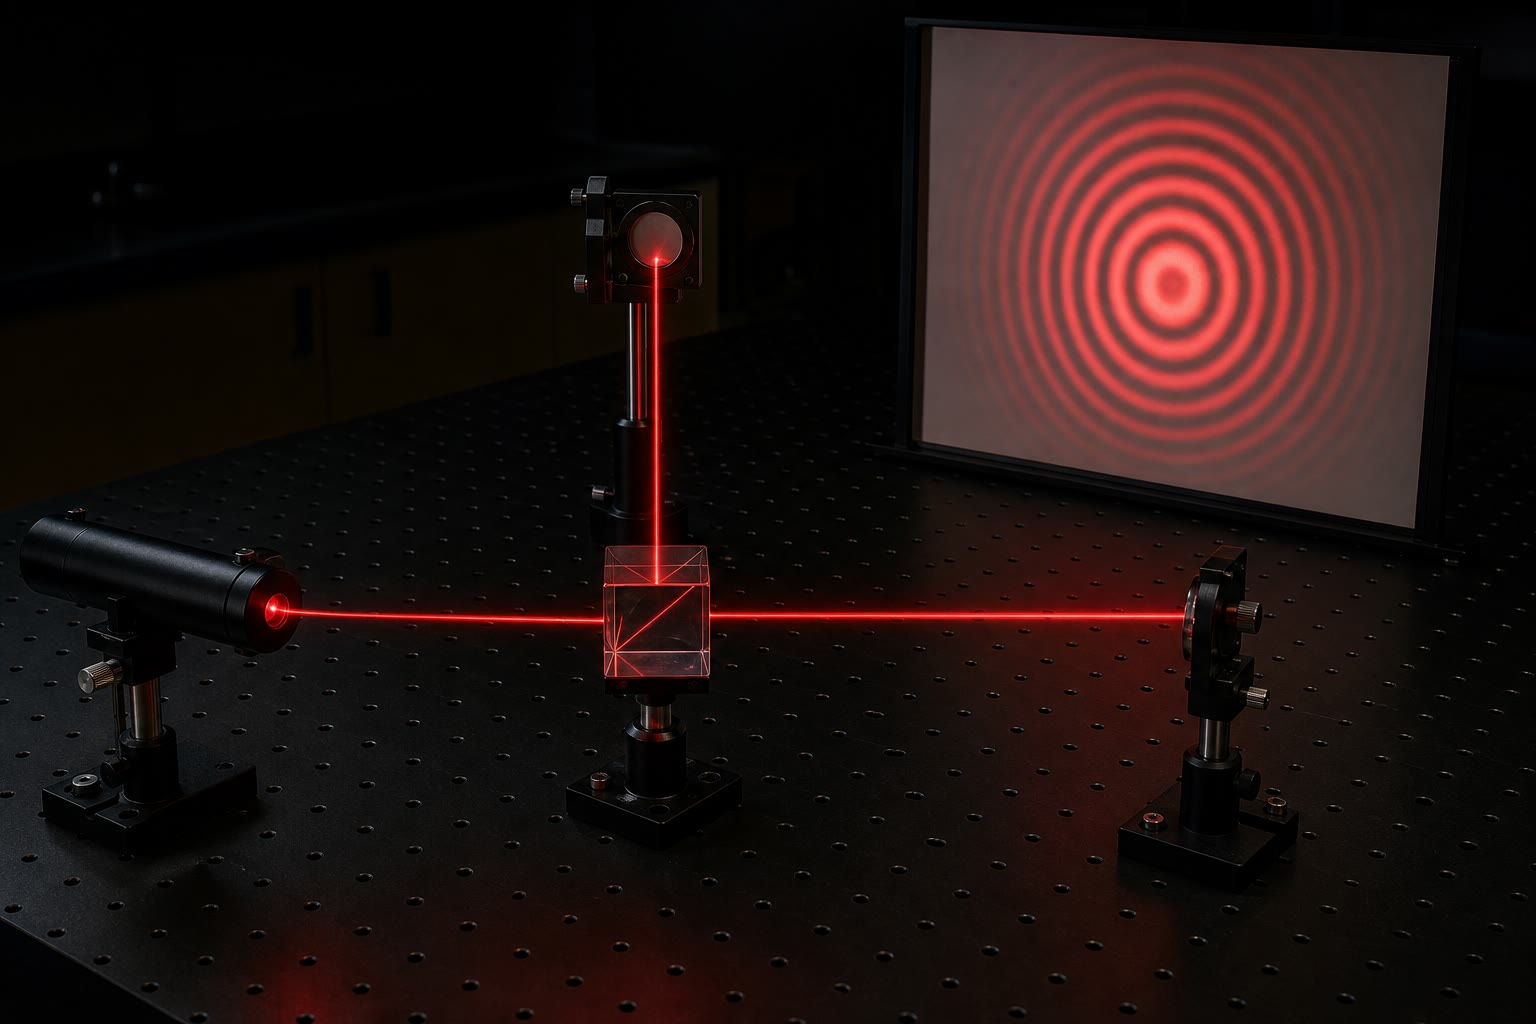
\includegraphics[width=0.58\linewidth]{images/book4/ai/b4-20-michelson-lab.jpg}

{\small Un \omterm{def:b2:michelson:instrument}{interferómetro de Michelson} en un banco de prácticas: láser, cubo separador, dos espejos y, en la pantalla, los \omterm{prop:b2:michelson:rings}{anillos de igual inclinación} de la lámina de aire.}
\end{omfigure}

\begin{omfigure}
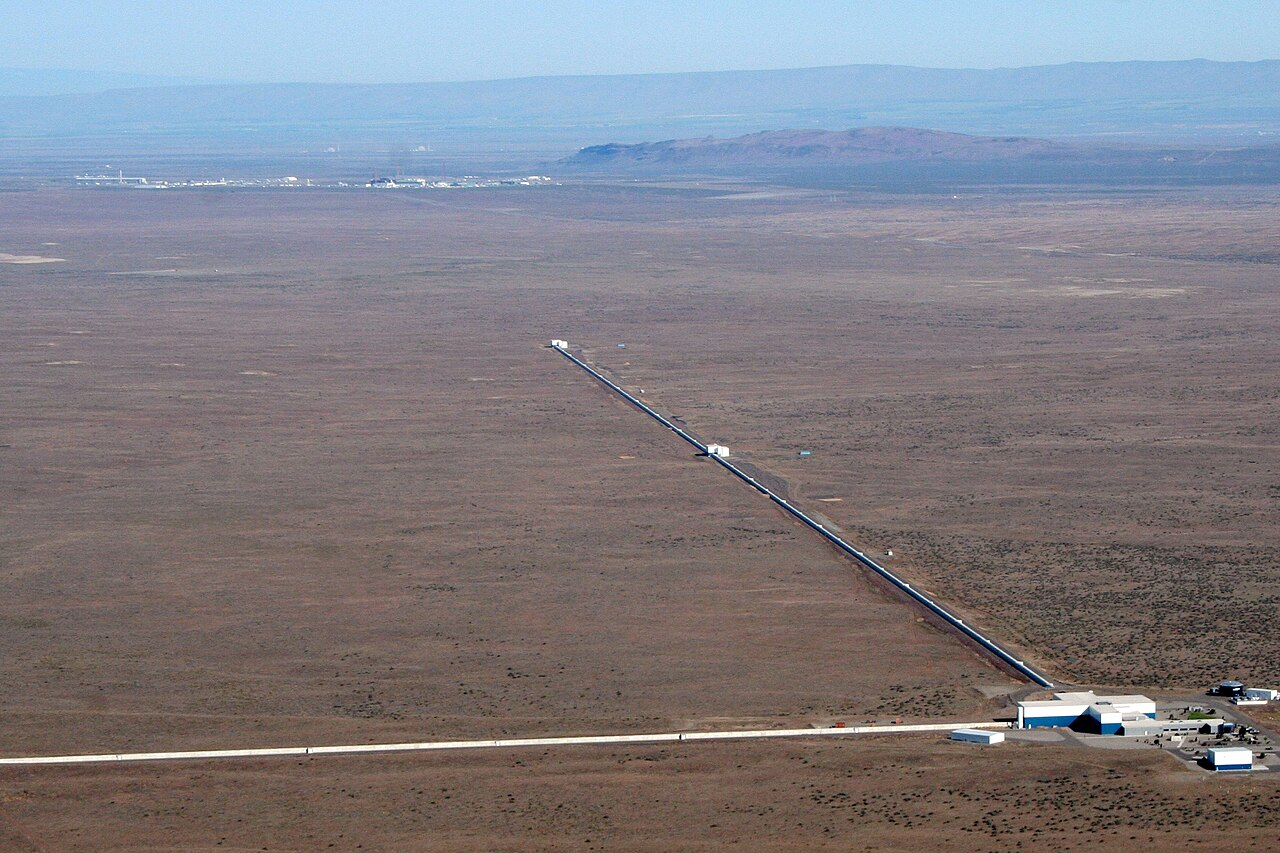
\includegraphics[width=0.6\linewidth]{images/book4/ligo-hanford-aerial.jpg}

{\small El interferómetro LIGO de Hanford: un \omterm{def:b2:michelson:instrument}{interferómetro de Michelson} con brazos de cuatro kilómetros que en 2015 registró un cambio de longitud de brazo de una milésima del diámetro de un protón --- el paso de una onda gravitacional (LIGO Laboratory).}
\end{omfigure}

\section{Problema: el doblete del sodio y el índice del aire}

\begin{problem}[{Problema de fin de semana --- una sesión completa de medidas
con un interferómetro de Michelson: encontrar el contacto, leer longitudes, desdoblar
la raya amarilla y pesar el aire}]
\label{pb:b2:michelson:1}

El interferómetro tiene un tornillo micrométrico que lee \qty{1}{\micro m}; la
lámpara de sodio da $\lambda_1 = \qty{589.0}{nm}$ y $\lambda_2 = \qty{589.6}{nm}$ con
intensidades $2 : 1$; también se dispone de una lámpara blanca y de un láser de He--Ne (\qty{632.8}{nm}).

\medskip
\noindent\textbf{Parte I --- Puesta a punto.}
\begin{enumerate}
  \item Con el láser, la estudiante ve en una tarjeta dos manchas de los dos brazos;
        las superpone con los tornillos de inclinación y ve entonces
        franjas rectas: ¿de qué configuración se trata, y qué dice
        su separación sobre la inclinación residual (separación de \qty{2}{mm})?
  \item Al girar los tornillos de inclinación, las franjas se curvan y luego se vuelven
        anillos: ¿por qué aparecen anillos, y dónde está ahora $M_1'$?
  \item Traslada el espejo y cuenta $158$ anillos tragados por
        el centro: desplazamiento; ¿en qué sentido cambia $e$?
  \item Al seguir, los anillos se separan y la mancha central crece
        hasta llenar el campo: ¿qué ha alcanzado? La lámpara de sodio
        sustituye al láser y no ve nada especial: ¿por qué no, y
        por qué muestra la luz blanca una franja central brillante flanqueada por
        franjas coloreadas en ese punto?
  \item Inclina muy ligeramente $M_1$ en el contacto y ve, con luz
        blanca, franjas rectas coloreadas: explíquese, y dígase cuántas
        puede esperar a cada lado de la blanca.
  \item Las manchas del láser miden \qty{10}{mm} de ancho y quiere diez anillos
        en el campo de una lente de $f = \qty{20}{cm}$ ($\lambda = \qty{632.8}{nm}$):
        espesor $e$ necesario (úsese el radio del $k$-ésimo anillo).
  \item ¿Por qué debe ser paralela la \omterm{def:b2:michelson:instrument}{lámina compensadora} a la separadora,
        y qué vería con luz blanca si se quitara?
\end{enumerate}

\medskip
\noindent\textbf{Parte II --- El doblete.}
\begin{enumerate}[resume]
  \item Partiendo del contacto con la lámpara de sodio, aumenta $e$:
        el contraste de los anillos cae, se anula y vuelve. Espesor de la
        primera desaparición; y de la $n$-ésima.
  \item Registra $12$ desapariciones entre $e = \qty{0.15}{mm}$ y
        $e = \qty{3.35}{mm}$ (la primera y la última leídas en el tornillo):
        $\Delta\lambda$; precisión si cada lectura es buena hasta \qty{5}{\micro m}.
  \item Órdenes $p_1$ y $p_2$ de las dos rayas en la primera
        desaparición; y en el primer retorno del contraste pleno.
  \item Contraste mínimo en una desaparición, dada la razón de
        intensidades $2 : 1$ (quedan las franjas de la raya más débil).
  \item ¿Cuántas desapariciones puede contar antes de que la anchura
        natural de las rayas (\qty{0.02}{nm} cada una) lo borre todo?
  \item ¿Qué mostraría una lámpara con tres rayas igualmente separadas?
\end{enumerate}

\medskip
\noindent\textbf{Parte III --- El aire.}
Se coloca en un brazo una cubeta de longitud $\ell = \qty{5.00}{cm}$ con ventanas de vidrio
y se hace el vacío; se deja entrar aire despacio mientras se cuentan las franjas
del láser.
\begin{enumerate}[resume]
  \item \omterm{thm:b2:two-wave-interference:formula}{Diferencia de camino} óptico creada al llenar la cubeta a
        \qty{1}{atm} si $n - 1 = \qty{2.9e-4}{}$; número de franjas.
  \item Cuenta $46$ franjas: su valor de $n - 1$.
  \item Solo deja entrar \qty{0.20}{bar}: franjas esperadas ($n - 1 \propto$
        presión).
  \item La sala se calienta \qty{3}{K} durante la medida, y los
        \qty{40}{cm} de aire libre de cada brazo cambian de índice en
        $-\qty{1e-6}{}$ por kelvin: deriva de franjas; ¿es un problema para
        la Parte II? ¿Y para la Parte III?
  \item ¿Por qué no desplazan la medida las ventanas de la cubeta (están
        ahí durante toda la cuenta)?
  \item Se repite el experimento con CO$_2$ ($n - 1 = \qty{4.5e-4}{}$):
        franjas con la cubeta llena; ¿cómo podría identificarse el gas solo
        a partir de la cuenta?
\end{enumerate}

\medskip
\noindent\textbf{Parte IV --- Límites.}
\begin{enumerate}[resume]
  \item El tornillo se lee a \qty{1}{\micro m}: precisión de una longitud
        medida contando franjas en \qty{1}{cm}, frente a la del tornillo
        solo.
  \item Una vibración de \qty{50}{nm} de amplitud a \qty{100}{Hz} sacude uno de los
        espejos: movimiento de las franjas; ¿qué ve el ojo y qué ve una
        cámara a $25$ imágenes por segundo?
  \item La frecuencia del láser deriva \qty{1e-8}{} en valor relativo
        durante una cuenta en $e = \qty{1}{cm}$: error en franjas.
  \item Un bloque patrón de \qty{10}{mm} está certificado con $\lambda/20$ por
        interferometría: precisión absoluta y relativa.
  \item ¿Por qué es el Michelson el instrumento de elección para longitudes, y
        la red (capítulo siguiente) para espectros?
  \item Resúmanse las cuatro magnitudes medidas (una longitud, el desdoblamiento
        de un doblete, un índice y una \omterm{prop:b2:scalar-light-model:coherence}{longitud de coherencia}) y la observación
        de franjas que dio cada una.
\end{enumerate}
\end{problem}
